%=====================================================================%
% DOCUMENT DEFINITION
%=====================================================================%


\documentclass[12pt]{article}

\usepackage[english]{babel}

\usepackage{subcaption}

\usepackage{gensymb}

\usepackage{setspace}
\onehalfspacing

\usepackage[
    a4paper,
    top=2cm,
    bottom=2cm,
    left=2cm,
    right=2cm,
    marginparwidth=1.75cm
]{geometry}

\usepackage[skip=8pt plus1pt, indent=20pt]{parskip}

% inserting images
\usepackage{graphicx}
\usepackage{float}
\graphicspath{{images/}}

% references
\usepackage{csquotes}
\usepackage[
    backend=biber,
    style=numeric-comp,
    sorting=none
]{biblatex}
\addbibresource{references.bib}


% math
\usepackage{amsmath}
\usepackage{empheq}

% tables
\usepackage{booktabs}

% color
\usepackage{xcolor}

% dummy text
\usepackage{lipsum}


%=====================================================================%
% DOCUMENT
%=====================================================================%
\setlength{\parindent}{0pt} 


\begin{document}

%=====================================================================%
% TITLE PAGE
%=====================================================================%

\begin{titlepage}

\centering
\singlespacing

% ------------------------------------------------
% UNIVERSITY LOGO
% ------------------------------------------------

\includegraphics[width=0.70\textwidth]{bmelogo.png}

\vspace{0.4cm}

{\Large\bfseries
Budapest University of Technology and Economics\par}

\vspace{0.15cm}

{\Large Faculty of Natural Sciences\par}

% ------------------------------------------------
% TITLE
% ------------------------------------------------

\vspace{3.3cm}

{\LARGE\bfseries
M4 - Digital circuits \\
\par}

\vspace{0.3cm}

{\Large Lab report\par}

% ------------------------------------------------
% DATE
% ------------------------------------------------

\vspace{2.6cm}

{\Large 18/11/2026\par}

% ------------------------------------------------
% LAB RESPONSIBLE
% ------------------------------------------------

\vspace{2.5cm}

{\Large
\underline{Lab responsible}\\[-0.05cm]
\textbf{Viktor Farkas}
\par}

% ------------------------------------------------
% STUDENTS
% ------------------------------------------------

\vfill

\begin{minipage}[t]{0.47\textwidth}
    \centering

    {\Large {Student}\par}

    \vspace{0.1cm}

    {\bfseries
    Abigél ORTUTAY (UGHRKC)\par}
     {\normalsize
    Physics-engineering BSc 3rd year\par}
    {\normalsize
    abico.ortutay@gmail.com}
    
\end{minipage}
\hfill
\begin{minipage}[t]{0.47\textwidth}
    \centering

    {\Large {Student}\par}
   

    \vspace{0.1cm}

    {\bfseries
    Hanna ERTL (SPH4U7)\par}
    {\normalsize
    Physics-engineering BSc 3rd year\par}
    {\normalsize
    hannavedaertl@gmail.com}
    
    
\end{minipage}

\vspace{1.3cm}

\end{titlepage}


%=====================================================================%
% REPORT STARTS HERE
%=====================================================================%
\begin{abstract}
    \noindent In this work, the operation and characteristics of digital circuits were investigated, and the observed results are presented. An unknown logic gate was identified by determining its truth table, and then the effect of connecting its inputs together were examined. The rise and fall times of the circuit were measured using an oscilloscope. 

    The operation of a BCD counter is investigated by recording its counting sequence and examining the individual output signals. An extended circuit is constructed with a decoder and a seven-segment display to demonstrate the decimal counting. Finally, the required resistance and minimum power rating of the series resistors of the display are calculated. 
\end{abstract}

\section{Theoretical introduction}
Digital circuits implement logical relationships that form the foundation of computing, 
instrumentation, and automated control systems. They are built from logic gates using binary 
logic, 0 for "no" in the false state, and 1 for "yes" in the true state. In semiconductor integrated
circuits (ICs) this logic gate is implemented in two ways using bipolar or MOS transistors: 
Transistor - Transistor Logic (TTL) and Complementary Metal-Oxide Semiconductor (CMOS).

For the real world application of these circuits - for example in the measurement we completed in 
this laboratory exercise - the voltages below approximately 0.8 V represent the false state (low logic), 
while voltages above approximately 2.4 V represent true state (high logic).

Sequential networks can be used to implement time dependent logic circuits, where the output doesn't depend 
only on the instantaneous input, but also on the past internal states. The two types of sequential networks are: 
asynchronous networks and synchronous networks. Asynchronous networks have instantaneous change in their output 
when the input changes, and synchronous networks use an enabling clock signal to read the input.

Flip-flops are used to compose sequential circuits, these serve as 1-bit primary memory components. The different 
types of flip-flops are:
\begin{itemize}
\item RS flip-flop: with set (S) and reset (R) pins. The S = 1, R = 1 combination is forbidden, as we cannot 
set and reset at the same time.
\item JK flip-flop: to solve the issue of the forbidden state of the RS flip-flop the output of the JK flip-flop 
toggles to Q negate when J = 1, K = 1 is detected. This flip-flop is synchronous, with a clock signal input 
pin as well.
\item T flip-flop: By connecting the J and K pins of the JK fip-flop together we get a configuration of two 
input pins of T (toggle) and a clock signal.
\item D flip-flop: this configuration introduces a time delay (D) using a control signal between the input 
and the output signal of the flip-flop.
\end{itemize}

Utilising flip-flop units we can form counter circuits of synchronous and asynchronous kind. In a asynchronous 
counter the connected flip-flops are driven sequentially after each other, the next flip flop receives its triggering 
signal from the previous flip-flop in the arrangement; hence, their operation does not occur at the same time. 
In synchronous counters they receive the triggering signal simultaneously, which causes them to toggle at the same 
instant. Counting up, down, or up and down depends on storage and addition, since each flip-flop can store 1 binary bit, a composition of 
$n$ flip-flops can store $2^n$ bits. When a counter reaches its maximum capacity, it resets, continuing the pulse 
count from the beginning. The pulse count can be encoded in binary, decimal, Gray code, and Johnson code.

The three output types of a digital circuit can be the following: totem-pole output, open-collector output (OC), 
and three-state output. Totem-pole outputs allow for high and low levels, building on this the three-state output 
also has a high impedance output where both internal switches are switched off. The open-collector output uses 
an active switch to pull the output down to the low level, requiring an external pull up resistor to pull the 
output up to the high level. Real life applications introduce dynamic performance limitations of: propegation delay, 
rise and fall time, pulse duration (width), as well as strict temporal rules to follow such as the setup time, and 
the hold time. 

\section{Measurement tools}
For this measurement, we used the following list of tools:
\begin{itemize}
\item TI SN74LS00 PC 8451 Logic Gate
\item SIGLENT SPD3303C Programmable DC Power Supply
\item HAMEG HM 8011-3 Digital multimeter
\item SIGLENT SDS 1072CML Digital storage oscilloscope
\item SN74LS390 BCD Counter
\item HDSP5731 7-segment display
\item Banana cables (4 pieces)
\item Crocodile clips (4 pieces)
\item Jumping wires (20 pieces)
\item 270 k$\Omega$ resistor (7 pieces)
\end{itemize}

\newpage \section{Measurement setup}

\pagebreak\section{Measurements}

\subsection{Examination of a logic gate (black-box measurement)}

\subsubsection{Determining the type of the logic gate}
We investigated the operation of a logic gate. The integrated circuit contains 4 logic gates, and one of them was studied. A 5 V supply voltage was applied to the Vcc (pin 14) relative to GND (pin 7).
In order to examine the behavior of the gate, the two input values (pin 1 and pin 2) were set to either 0 V or 5 V in all four possible combinations. The corresponding output of the system (pin 3) was measured with a multimeter. The different input voltage combinations with the corresponding output values are summarized in Table~\ref{tab:logicgate1}.
\begin{table}[ht]
    \centering
    \begin{tabular}{l|c|c|c|c}
    \hline
    \textbf{Input 1 (PIN1)} & GND & 5 V & 5 V & GND \\ \hline
    \textbf{Input 2 (PIN2)} & 5 V  & GND & 5 V & GND \\ \hline
    \textbf{Output} & 4.013 V & 4.016 V & 0.160 V & 4.038 V \\ \hline
    \end{tabular}
    \caption{Low and high state voltage responses of logic gate}
    \label{tab:logicgate1}
\end{table}

Based on the measurements, the high output level of the circuit was determined to be approximately 4.02 V, while the low level was approximately 0.16 V.

Since the output was low only when both inputs were high, and all other configurations yielded a high output, the observed behavior of the truth table shows that the investigated logic gate is a NAND type. 

\subsubsection{Connecting inputs 1 and 2 of the examined circuit}
Using the previous configuration, the two inputs of the NAND gate were connected together to examine the change in the behavior of the resulting logic gate. The measurement configuration is shown in Fig.~\ref{fig:task1_B}.
\begin{figure}[H]
    \centering
    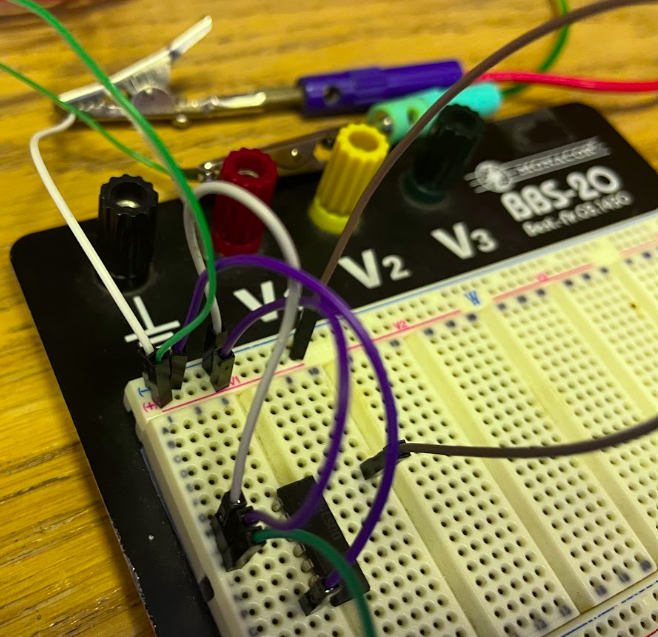
\includegraphics[width=0.3\linewidth]{task1_b.png}
    \caption{Connected input 1 and 2 of a logic gate.}
    \label{fig:task1_B}
\end{figure}

An input of 0 V (GND) resulted in a measured output voltage of 4.042 V, while for an input of 5 V, the corresponding output value was 0.160 V. Therefore, a low level input resulted in a high level output, and a high input produced a low output. 
These results demonstrate that connecting the two inputs of a NAND gate together results in a NOT gate behavior, which invert the applied logical input.

\subsubsection{Determining the rise and fall time of the output signal}
A 1 kHz square wave with a voltage range of 0-5 V was applied to the previously constructed circuit to determine the rise and fall times of its output signal. The function generator output was connected to PIN 1 and 2 of the logic gate. To measure the signals, a SIGLENT oscilloscope was used, with Channel 1 (Ch1) connected to the output of the logic gate (PIN 3), and Channel 2 (Ch2) was used to monitor the input signal. A 5 V supply voltage was applied to Vcc in this measurement as well.

The rise and fall times of the output signal were determined using the oscilloscope's measurement function. For the applied 1 kHz square wave, the measured rise and fall times were approximately 200-400 ns. At an input voltage of 5 V, the measured rise time was approximately 200 ns.  The measured rise and fall times fluctuated between 200 and 400 ns on the oscilloscope display, therefore, the values could only be determined approximately. The observed uncertainty may therefore be due to the limited measurement resolution and stability of the oscilloscope readings. 

The measured input and output waveforms are shown in Fig.~\ref{fig:risefall}. 

\begin{figure}[H]
    \centering
    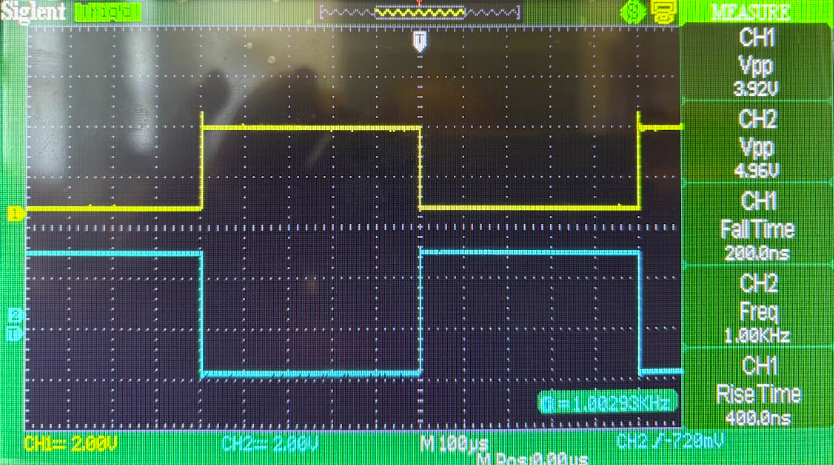
\includegraphics[width=0.5\linewidth]{image.png}
    \caption{Oscilloscope measurement of the input and output signals of the logic gate at 1 kHz.}
    \label{fig:risefall}
\end{figure}



\subsection{Examination of a BCD counter (SN74HCT390)}
After assembling the circuit according to the handout, the circuit's and its extended versions' behavior were examined.

\subsubsection{Truth table of the BCD counter}
A 1 Hz square wave with a voltage range of 0-5 V was applied to the circuit to examine its counting behavior. The observed output states are summarized in Table~\ref{tab:bcd_counter}.

\begin{table}[ht]
    \centering
    \begin{tabular}{c|c|c|c|c}
    \hline
    \textbf{Count} & $\mathbf{Q_A}$ & $\mathbf{Q_B}$ & $\mathbf{Q_C}$ & $\mathbf{Q_D}$ \\ \hline
    0 &0 &0 &0 &0 \\ \hline
    1 &1 &0 &0 &0 \\ \hline
    2 &0 &1 &0 &0 \\ \hline
    3 &1 &1 &0 &0 \\ \hline
    4 &0 &0 &1 &0 \\ \hline
    5 &1 &0 &1 &0 \\ \hline
    6 &0 &1 &1 &0 \\ \hline
    7 &1 &1 &1 &0 \\ \hline
    8 &0 &0 &0 &1 \\ \hline
    9 &1 &0 &0 &1 \\ \hline
    \end{tabular}
    \caption{Measured truth table of the BCD counter.}
    \label{tab:bcd_counter}
\end{table}

The obtained results show that the circuit operates as a BCD counter, representing the decimal numbers from 0 to 9 with the use of four binary outputs. It is observed that each incoming clock pulse increases the stored count by one, as expected. After reaching 9, the counter returned to 0, and the counting sequence was repeated.

\subsubsection{Examining individual outputs and operation}
To investigate the behavior of the individual outputs of the BCD counter, a 1 kHz square wave was applied to the circuit. The output signals $Q_A$, $Q_B$, $Q_C$ and $Q_D$ were examined using an oscilloscope.  

\begin{figure}[H]
    \centering
    \begin{subfigure}[t]{0.48\textwidth}
        \centering
        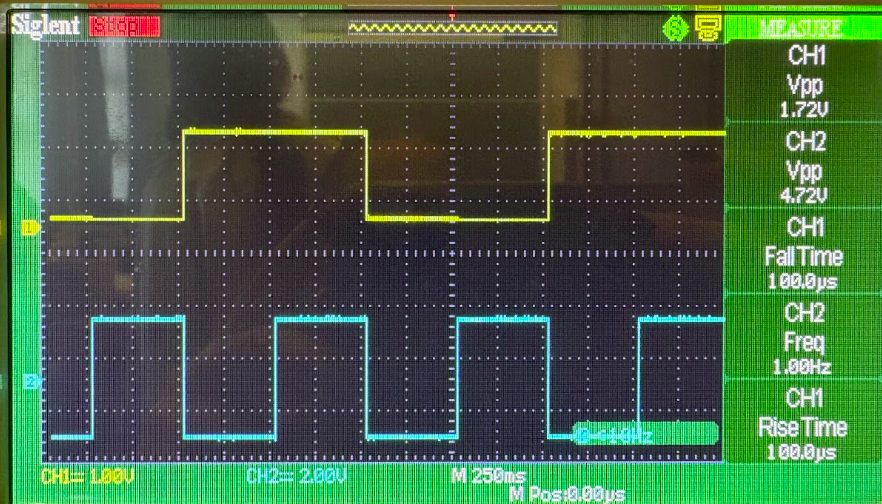
\includegraphics[width=\linewidth]{QA.png}
        \caption{$Q_A$}
        \label{fig:QA}
    \end{subfigure}
    \hfill
    \begin{subfigure}[t]{0.48\textwidth}
        \centering
        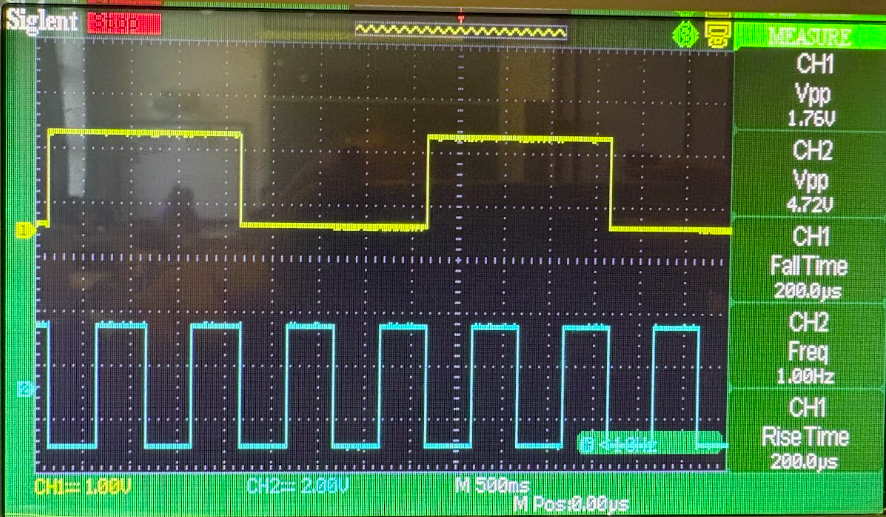
\includegraphics[width=\linewidth]{QB.png}
        \caption{$Q_B$}
        \label{fig:QB}
    \end{subfigure}

    \vspace{0.3cm}

    \begin{subfigure}[t]{0.48\textwidth}
        \centering
        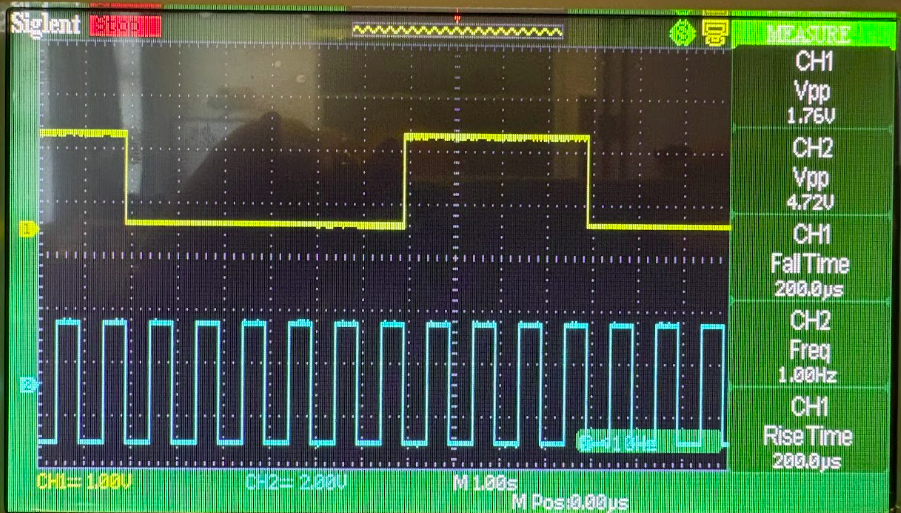
\includegraphics[width=\linewidth]{QC.png}
        \caption{$Q_C$}
        \label{fig:QC}
    \end{subfigure}
    \hfill
    \begin{subfigure}[t]{0.48\textwidth}
        \centering
        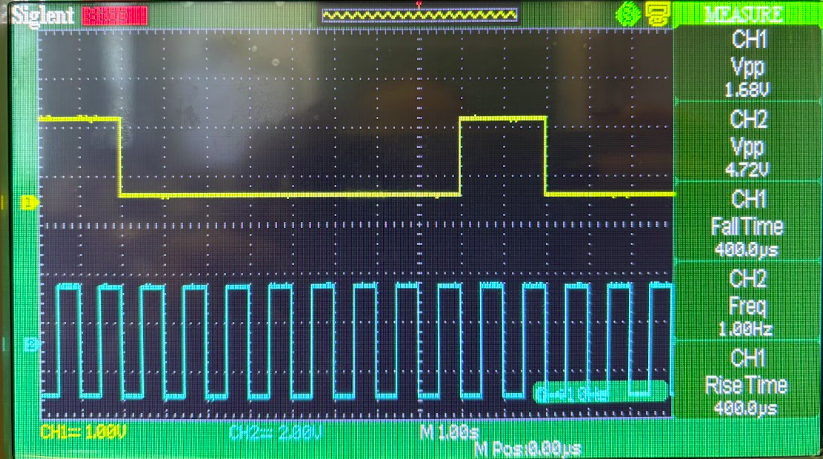
\includegraphics[width=\linewidth]{QD.png}
        \caption{$Q_D$}
        \label{fig:QD}
    \end{subfigure}

    \caption{Oscilloscope measurements of the individual
    outputs of the BCD counter at an input frequency
    of 1 kHz.}
    \label{fig:bcd_outputs}
\end{figure}

In each case, on Channel 1 of the oscilloscope, we can see the individual counter outputs. The switching patters differ according to the counting sequence of the BDC. On Channel 2, the input square wave is visible, which remained the same throughout all four measurements, with a measured peak-to-peak voltage of approximately 4.72 V. The input pulses appeared increasingly dense in the oscilloscope screenshots due to changes in the horizontal time scale, not as changes in the input frequency.

The output $Q_A$ changes its state most frequently out of the four measurement values. It can be seen that one complete output cycle corresponds to two input clock cycles, therefore $Q_A$ has a frequency of approximately 500 Hz for the applied 1 kHz input. The other outputs change less frequently, according to the binary-coded counting sequence.

The output $Q_B$ generally remained low for two clock periods and high for two clock periods, visible on the oscilloscope picture. What is not seen on the oscilloscope picture is the behavior when the counting sequence returns from 9 to 0. According to the truth table of $Q_B$, in this case a longer low interval is observed, for four clock periods.

$Q_C$ remains high for four consecutive counts approximately, and $Q_D$ for two consecutive counts. Since $Q_C$ is high for 4 input clock periods, and low for 6 input clock periods, one complete output cycle requires approximately 10 input clock periods. Since a 1 kHz input frequency corresponds to a
\begin{equation}
    T = \frac{1}{f}=\frac{1}{1000}=0.001 ~\mathrm{seconds} = 1 ~\mathrm{ms}
\end{equation}
time period, we can calculate the corresponding $T_{Q_C}$ as:
\begin{equation}
    T_{Q_C}=10 \cdot 1 ~\mathrm{ms} = 10 ~\mathrm{ms}.
\end{equation}

From that we can obtain $f_{Q_c}$ as follows:
\begin{equation}
    f_{Q_C} = \frac{1}{0.01}=100 ~\mathrm{Hz}.
\end{equation}

The same calculation can be applied to the $Q_D$ response, which yields a $f_{Q_D}$ = 100 Hz as well. Therefore, we obtain that both outputs have the same frequency but different high and low durations, which is consistent with the truth table, as $Q_C$ is high at counts 4-7, while $Q_D$ is high at counts 8-9.  

\subsubsection{Examination of counter outputs and seven-segment display}
The previously constructed BCD counter circuit was extended with an SN7447 decoder and an HDSP-5731 seven-segment display, according to the circuit diagram provided in the handout. A 1 Hz square wave with a voltage range of 0--5 V was applied to the input. 

The decoder converts the binary-coded output of the counter into signals controlling the individual segments of the display. Consequently, the corresponding decimal digit is displayed at each counting step.


\begin{figure}[H]
    \centering

    \begin{subfigure}[t]{0.18\textwidth}
        \centering
        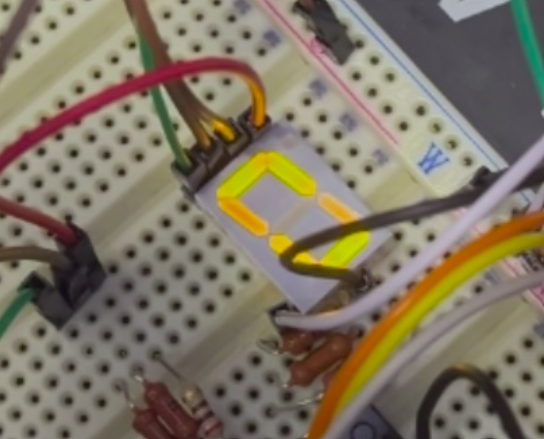
\includegraphics[width=\linewidth,height=2.5cm]{digit0.png}
        \caption{0}
    \end{subfigure}
    \hfill
    \begin{subfigure}[t]{0.18\textwidth}
        \centering
        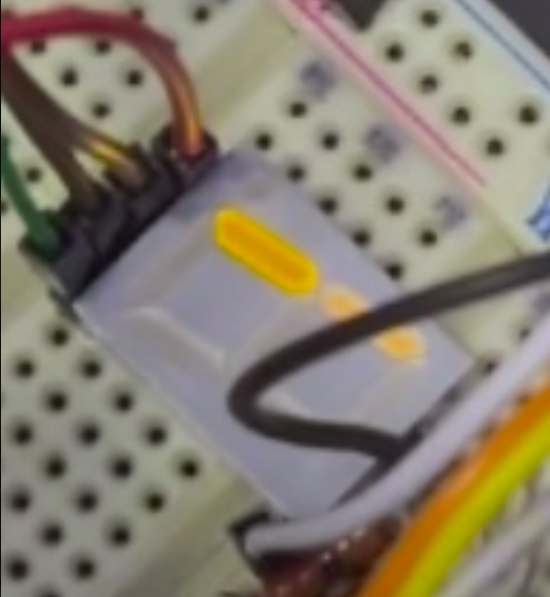
\includegraphics[width=\linewidth,height=2.5cm]{digit1.png}
        \caption{1}
    \end{subfigure}
    \hfill
    \begin{subfigure}[t]{0.18\textwidth}
        \centering
        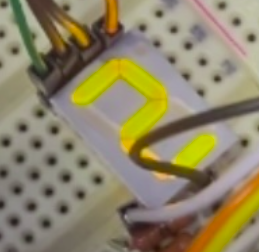
\includegraphics[width=\linewidth,height=2.5cm]{digit2.png}
        \caption{2}
    \end{subfigure}
    \hfill
    \begin{subfigure}[t]{0.18\textwidth}
        \centering
        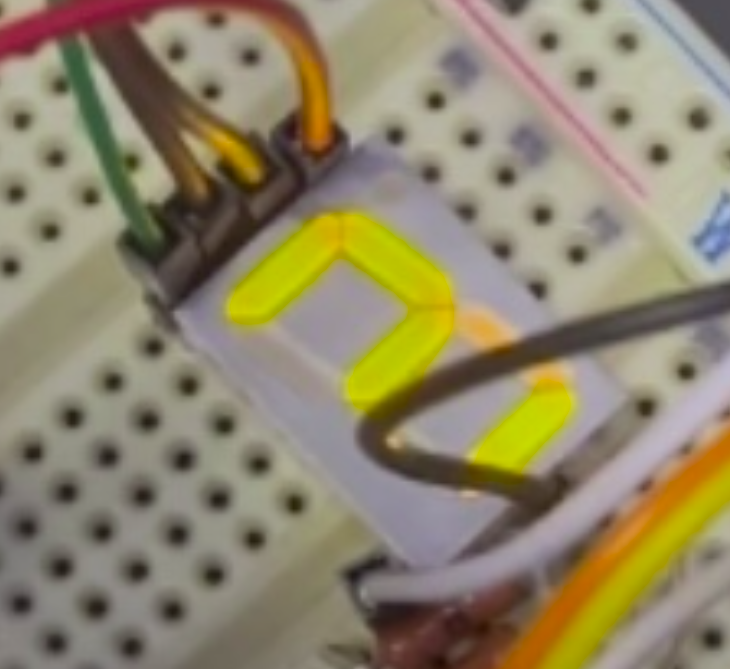
\includegraphics[width=\linewidth,height=2.5cm]{digit3.png}
        \caption{3}
    \end{subfigure}
    \hfill
    \begin{subfigure}[t]{0.18\textwidth}
        \centering
        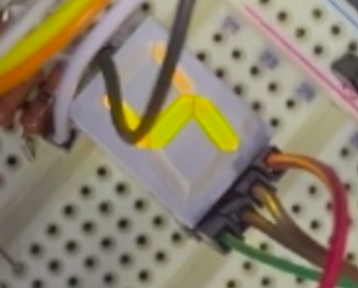
\includegraphics[width=\linewidth,height=2.5cm]{digit4.png}
        \caption{4}
    \end{subfigure}

    \par\vspace{0.3cm}

    \begin{subfigure}[t]{0.18\textwidth}
        \centering
        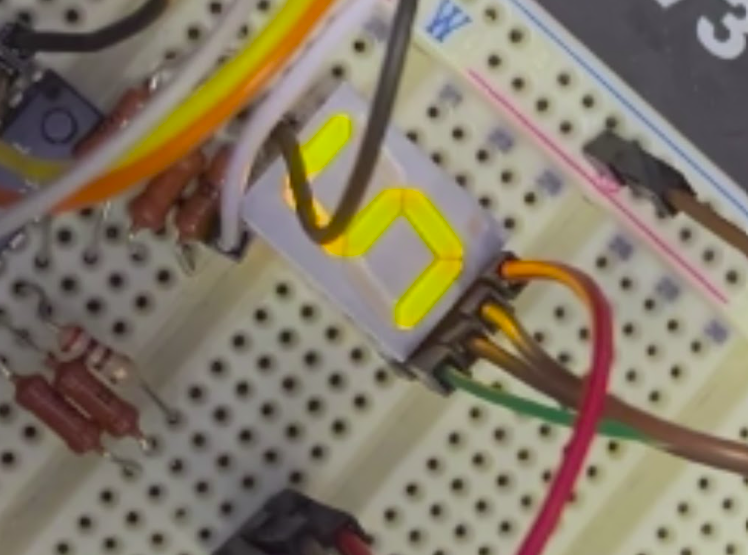
\includegraphics[width=\linewidth,height=2.5cm]{digit5.png}
        \caption{5}
    \end{subfigure}
    \hfill
    \begin{subfigure}[t]{0.18\textwidth}
        \centering
        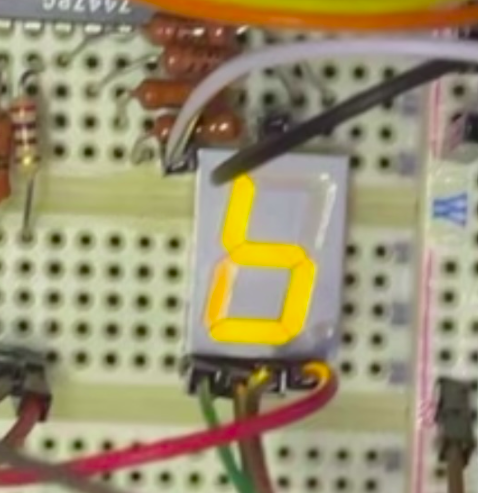
\includegraphics[width=\linewidth,height=2.5cm]{digit6.png}
        \caption{6}
    \end{subfigure}
    \hfill
    \begin{subfigure}[t]{0.18\textwidth}
        \centering
        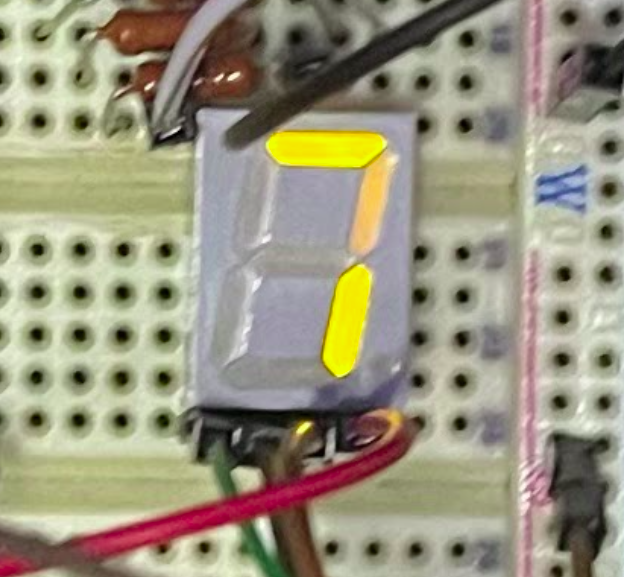
\includegraphics[width=\linewidth,height=2.5cm]{digit7.png}
        \caption{7}
    \end{subfigure}
    \hfill
    \begin{subfigure}[t]{0.18\textwidth}
        \centering
        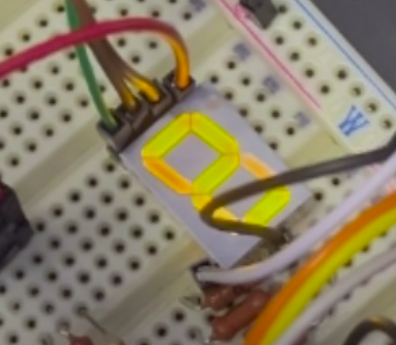
\includegraphics[width=\linewidth,height=2.5cm]{digit8.png}
        \caption{8}
    \end{subfigure}
    \hfill
    \begin{subfigure}[t]{0.18\textwidth}
        \centering
        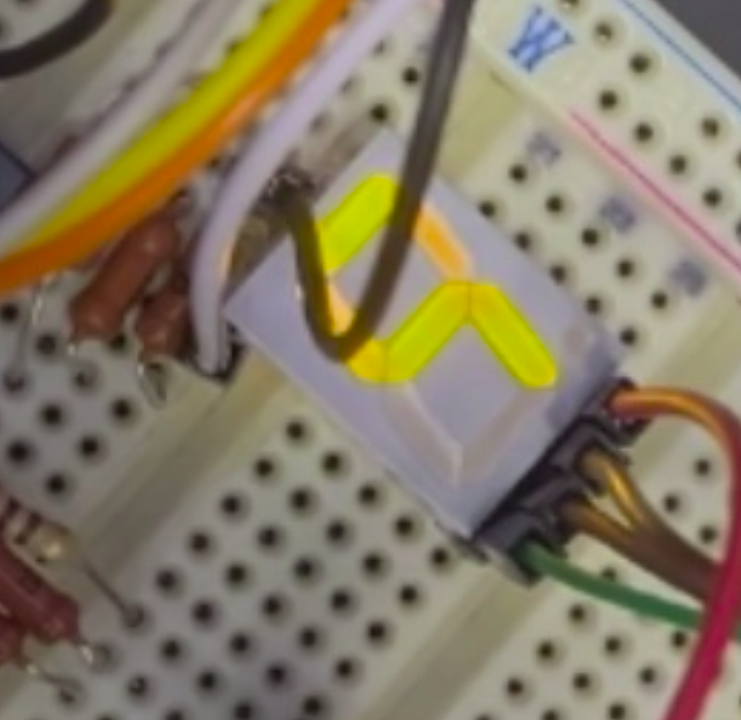
\includegraphics[width=\linewidth,height=2.5cm]{digit9.png}
        \caption{9}
    \end{subfigure}

    \caption{Observed decimal digits displayed by the seven-segment display during the counting sequence.}
    \label{fig:7segment_digits}
\end{figure}

During the measurement, the display showed the decimal digits from 0 to 9, and the counting sequence continuously restarted from 0. The observations shown in Fig.~\ref{fig:7segment_digits} confirm the expected operation of the BCD counter and decoder.

\begin{figure}
    \centering
    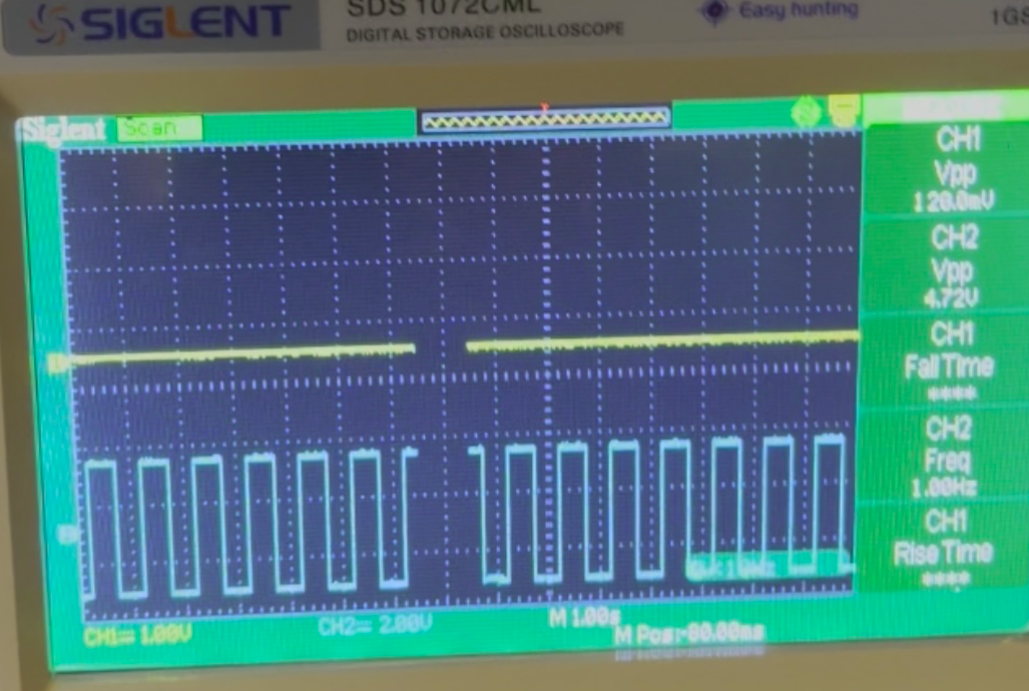
\includegraphics[width=0.5\linewidth]{7displayosci.png}
    \caption{Oscilloscope measurement during the operation of the seven-segment display circuit.}
    \label{fig:scope_display}
\end{figure}

Fig.~\ref{fig:scope_display} displays the corresponding signals during the measurement. Channel 2 displayed a periodic square-wave signal, while Channel 1 remained approximately constant over most of the observed interval. Short interruptions were visible in both signals at approximately the same position, which shifted together.

\subsubsection{Justification of the use of 270 $\Omega$ series resistors}
The final circuit used series resistors of 270 $\Omega$ for the seven-segment display. The LED forward voltage was 1.8 V, with a current of 10 mA. A 5 V high level was expected at the counter output.

Because of the series configuration, the voltage across the resistor is:
\begin{equation}
    U = 5 - 1.8 = 3.2 ~\mathrm{V}.
\end{equation}

For a current of 10 mA, the required resistance is
\begin{equation}
    R = \frac{U}{I}=\frac{3.2}{0.01}=320~\Omega. 
\end{equation}

For series resistors with a resistance of 270 $\Omega$, the current is 
\begin{equation}
    I = \frac{3.2}{270}=0.01185~\mathrm{A} = 11.85~\mathrm{mA}.
\end{equation}

This result shows that the specified resistor value results in a higher current than the assumed 10 mA value.

The minimum power rating of the resistor can be calculated by the power dissipated by each resistor:
\begin{equation}
    P = \frac{U^2}{R}=\frac{3.2^2}{270}=0.038~\mathrm{W}.
\end{equation}

This calculation yields that the minimum required power rating is approximately 38 mW. Therefore, we need a resistor rated above this value. 

\section{Conclusion}
During the laboratory, the operation of digital logical circuits were successfully investigated. In the first measurement, based on the truth table we have determined that the examined logic gate was a NADND gate, with high and low output levels of 4.02 V and 0.16 V, respectively. By connecting its inputs together, we obtained a circuit exhibiting a NOT gate behavior, meeting the expectation. The measured fall and rise times were approximately 200-400 ns, with the limited precision coming from fluctuations in the oscilloscope readings.

A BCD counter was also examined, and the measured output states followed the expected counting sequence from 0 to 9, repeating after each cycle. The extended circuit with the seven-segment display also operated as expected, displaying decimal digits from 0 to 9.

The series resistor calculations yielded a resistance of 320 $\Omega$ for the 10 mA assumed current. For the 270 $\Omega$ resistors, the calculations resulted in a currenf of 11.85 mA, with a minimum power rating of 38 mW.

\nocite{*}
\printbibliography 
\end{document}